\section{Observations and Calculations}
	\begin{table}[H]
	\centering
	\resizebox{\columnwidth}{!}{%
	\begin{tabular}{|c|c|c|c|c|c|c|c|}
	\hline
	Drop no & Sl no & \begin{tabular}[c]{@{}c@{}}Free Fall\\ time   (s)\end{tabular} & Rise time (s) & \begin{tabular}[c]{@{}c@{}}Mean Free fall\\ time\end{tabular} & \begin{tabular}[c]{@{}c@{}}Mean Rise\\ time\end{tabular} & \begin{tabular}[c]{@{}c@{}}Mean free fall velocity\\ $(v_f = \sfrac{L}{t_f}\times 10^{5})$\\ $(ms^{-1})$\end{tabular} & Voltage (V) \\ \hline
	\multirow{5}{*}{1} & 1 & 9.9 & 16.1 & \multirow{5}{*}{10.12} & \multirow{5}{*}{15.1} & \multirow{5}{*}{9.881} & \multirow{5}{*}{378} \\ \cline{2-4}
	 & 2 & 10.4 & 14.6 &  &  &  &  \\ \cline{2-4}
	 & 3 & 10.3 & 14.8 &  &  &  &  \\ \cline{2-4}
	 & 4 & 10.3 & 14.2 &  &  &  &  \\ \cline{2-4}
	 & 5 & 9.7 & 15.8 &  &  &  &  \\ \hline
	\multirow{5}{*}{2} & 1 & 8.6 & 13.7 & \multirow{5}{*}{8.56} & \multirow{5}{*}{13.84} & \multirow{5}{*}{11.682} & \multirow{5}{*}{450} \\ \cline{2-4}
	 & 2 & 8.1 & 13.9 &  &  &  &  \\ \cline{2-4}
	 & 3 & 8.7 & 14.9 &  &  &  &  \\ \cline{2-4}
	 & 4 & 9 & 13.3 &  &  &  &  \\ \cline{2-4}
	 & 5 & 8.4 & 13.4 &  &  &  &  \\ \hline
	\multirow{5}{*}{3} & 1 & 10.3 & 7 & \multirow{5}{*}{10.14} & \multirow{5}{*}{6.4} & \multirow{5}{*}{9.862} & \multirow{5}{*}{343} \\ \cline{2-4}
	 & 2 & 10 & 6.4 &  &  &  &  \\ \cline{2-4}
	 & 3 & 10.1 & 6.2 &  &  &  &  \\ \cline{2-4}
	 & 4 & 10.1 & 6.2 &  &  &  &  \\ \cline{2-4}
	 & 5 & 10.2 & 6.2 &  &  &  &  \\ \hline
	\multirow{5}{*}{4} & 1 & 11.4 & 7 & \multirow{5}{*}{11.26} & \multirow{5}{*}{6.84} & \multirow{5}{*}{8.881} & \multirow{5}{*}{500} \\ \cline{2-4}
	 & 2 & 11.2 & 6.6 &  &  &  &  \\ \cline{2-4}
	 & 3 & 11.3 & 6.8 &  &  &  &  \\ \cline{2-4}
	 & 4 & 11 & 7.1 &  &  &  &  \\ \cline{2-4}
	 & 5 & 11.4 & 6.7 &  &  &  &  \\ \hline
	\multirow{5}{*}{5} & 1 & 10.6 & 2.5 & \multirow{5}{*}{10.842} & \multirow{5}{*}{2.5} & \multirow{5}{*}{9.223} & \multirow{5}{*}{484} \\ \cline{2-4}
	 & 2 & 11.2 & 2.3 &  &  &  &  \\ \cline{2-4}
	 & 3 & 10.9 & 2.4 &  &  &  &  \\ \cline{2-4}
	 & 4 & 11.11 & 2.6 &  &  &  &  \\ \cline{2-4}
	 & 5 & 10.4 & 2.7 &  &  &  &  \\ \hline
	\multirow{5}{*}{6} & 1 & 19.7 & 8.9 & \multirow{5}{*}{19.92} & \multirow{5}{*}{8.36} & \multirow{5}{*}{5.020} & \multirow{5}{*}{400} \\ \cline{2-4}
	 & 2 & 20.4 & 7.7 &  &  &  &  \\ \cline{2-4}
	 & 3 & 18.9 & 8.3 &  &  &  &  \\ \cline{2-4}
	 & 4 & 20.4 & 8.7 &  &  &  &  \\ \cline{2-4}
	 & 5 & 20.2 & 8.2 &  &  &  &  \\ \hline
	\multirow{5}{*}{7} & 1 & 16.2 & 10.6 & \multirow{5}{*}{16.54} & \multirow{5}{*}{9.26} & \multirow{5}{*}{6.046} & \multirow{5}{*}{410} \\ \cline{2-4}
	 & 2 & 16.8 & 9.9 &  &  &  &  \\ \cline{2-4}
	 & 3 & 15.8 & 9.6 &  &  &  &  \\ \cline{2-4}
	 & 4 & 16.9 & 8.1 &  &  &  &  \\ \cline{2-4}
	 & 5 & 17 & 8.1 &  &  &  &  \\ \hline
	\end{tabular}%
	}
	\caption{Dynamic Method Data}
	\label{tab:1}
\end{table}

	\begin{figure}[H]
		\centering
		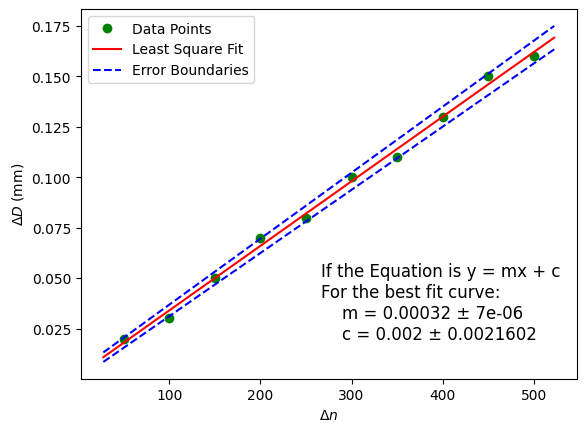
\includegraphics[width=0.4\textwidth]{graph_1.png}
		\caption{\textbf{Calibration Graph}}
		\label{graph:1}
	\end{figure}

	Average value of slope ($\mu$) is:




	% \subsection{Calibration of Lock-In Amplifier}

	% 	$U_F = 10.0V$ \hspace{1cm} $U_E = 6.2V$ \hspace{1cm} $U_G = 5.3V$

	% 	\begin{figure}[H]
	% 		\centering
	% 		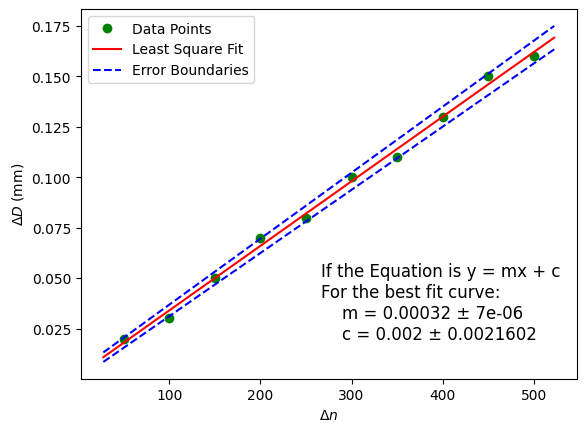
\includegraphics[width=0.37\textwidth]{graph_1.png}
	% 		\caption{\textbf{Graph for First dataset}}
	% 		\label{graph:1}
	% 	\end{figure}
		
	% 	\begin{table}[H]
	\centering
	\resizebox{\columnwidth}{!}{%
	\begin{tabular}{|c|c|c|c|c|c|c|c|}
	\hline
	Drop no & Sl no & \begin{tabular}[c]{@{}c@{}}Free Fall\\ time   (s)\end{tabular} & Rise time (s) & \begin{tabular}[c]{@{}c@{}}Mean Free fall\\ time\end{tabular} & \begin{tabular}[c]{@{}c@{}}Mean Rise\\ time\end{tabular} & \begin{tabular}[c]{@{}c@{}}Mean free fall velocity\\ $(v_f = \sfrac{L}{t_f}\times 10^{5})$\\ $(ms^{-1})$\end{tabular} & Voltage (V) \\ \hline
	\multirow{5}{*}{1} & 1 & 9.9 & 16.1 & \multirow{5}{*}{10.12} & \multirow{5}{*}{15.1} & \multirow{5}{*}{9.881} & \multirow{5}{*}{378} \\ \cline{2-4}
	 & 2 & 10.4 & 14.6 &  &  &  &  \\ \cline{2-4}
	 & 3 & 10.3 & 14.8 &  &  &  &  \\ \cline{2-4}
	 & 4 & 10.3 & 14.2 &  &  &  &  \\ \cline{2-4}
	 & 5 & 9.7 & 15.8 &  &  &  &  \\ \hline
	\multirow{5}{*}{2} & 1 & 8.6 & 13.7 & \multirow{5}{*}{8.56} & \multirow{5}{*}{13.84} & \multirow{5}{*}{11.682} & \multirow{5}{*}{450} \\ \cline{2-4}
	 & 2 & 8.1 & 13.9 &  &  &  &  \\ \cline{2-4}
	 & 3 & 8.7 & 14.9 &  &  &  &  \\ \cline{2-4}
	 & 4 & 9 & 13.3 &  &  &  &  \\ \cline{2-4}
	 & 5 & 8.4 & 13.4 &  &  &  &  \\ \hline
	\multirow{5}{*}{3} & 1 & 10.3 & 7 & \multirow{5}{*}{10.14} & \multirow{5}{*}{6.4} & \multirow{5}{*}{9.862} & \multirow{5}{*}{343} \\ \cline{2-4}
	 & 2 & 10 & 6.4 &  &  &  &  \\ \cline{2-4}
	 & 3 & 10.1 & 6.2 &  &  &  &  \\ \cline{2-4}
	 & 4 & 10.1 & 6.2 &  &  &  &  \\ \cline{2-4}
	 & 5 & 10.2 & 6.2 &  &  &  &  \\ \hline
	\multirow{5}{*}{4} & 1 & 11.4 & 7 & \multirow{5}{*}{11.26} & \multirow{5}{*}{6.84} & \multirow{5}{*}{8.881} & \multirow{5}{*}{500} \\ \cline{2-4}
	 & 2 & 11.2 & 6.6 &  &  &  &  \\ \cline{2-4}
	 & 3 & 11.3 & 6.8 &  &  &  &  \\ \cline{2-4}
	 & 4 & 11 & 7.1 &  &  &  &  \\ \cline{2-4}
	 & 5 & 11.4 & 6.7 &  &  &  &  \\ \hline
	\multirow{5}{*}{5} & 1 & 10.6 & 2.5 & \multirow{5}{*}{10.842} & \multirow{5}{*}{2.5} & \multirow{5}{*}{9.223} & \multirow{5}{*}{484} \\ \cline{2-4}
	 & 2 & 11.2 & 2.3 &  &  &  &  \\ \cline{2-4}
	 & 3 & 10.9 & 2.4 &  &  &  &  \\ \cline{2-4}
	 & 4 & 11.11 & 2.6 &  &  &  &  \\ \cline{2-4}
	 & 5 & 10.4 & 2.7 &  &  &  &  \\ \hline
	\multirow{5}{*}{6} & 1 & 19.7 & 8.9 & \multirow{5}{*}{19.92} & \multirow{5}{*}{8.36} & \multirow{5}{*}{5.020} & \multirow{5}{*}{400} \\ \cline{2-4}
	 & 2 & 20.4 & 7.7 &  &  &  &  \\ \cline{2-4}
	 & 3 & 18.9 & 8.3 &  &  &  &  \\ \cline{2-4}
	 & 4 & 20.4 & 8.7 &  &  &  &  \\ \cline{2-4}
	 & 5 & 20.2 & 8.2 &  &  &  &  \\ \hline
	\multirow{5}{*}{7} & 1 & 16.2 & 10.6 & \multirow{5}{*}{16.54} & \multirow{5}{*}{9.26} & \multirow{5}{*}{6.046} & \multirow{5}{*}{410} \\ \cline{2-4}
	 & 2 & 16.8 & 9.9 &  &  &  &  \\ \cline{2-4}
	 & 3 & 15.8 & 9.6 &  &  &  &  \\ \cline{2-4}
	 & 4 & 16.9 & 8.1 &  &  &  &  \\ \cline{2-4}
	 & 5 & 17 & 8.1 &  &  &  &  \\ \hline
	\end{tabular}%
	}
	\caption{Dynamic Method Data}
	\label{tab:1}
\end{table}

	% \subsection{Dataset II:}

	% 	$U_F = 9.2V$ \hspace{1cm} $U_E = 6.2V$ \hspace{1cm} $U_G = 6.5V$

	% 	\begin{table}[H]
	\centering
	\resizebox{\columnwidth}{!}{%
	\begin{tabular}{|c|c|c|c|c|c|c|}
	\hline
	Drop no & Sl no & \begin{tabular}[c]{@{}c@{}}Free Fall\\ time (s)\end{tabular} & \begin{tabular}[c]{@{}c@{}}Mean Free fall\\ time ($t_f$) (s)\end{tabular} & \begin{tabular}[c]{@{}c@{}}Mean free fall velocity\\ $(v_f = \sfrac{L}{t_f}$\\ $\times 10^{5}\;(ms^{-1})$\end{tabular} & Balancing voltage(V) & Voltage (V) \\ \hline
	\multirow{5}{*}{1} & 1 & 4.9 & \multirow{5}{*}{4.64} & \multirow{5}{*}{0.0002} &  & \multirow{5}{*}{238} \\ \cline{2-3} \cline{6-6}
	 & 2 & 4.6 &  &  & 238 &  \\ \cline{2-3} \cline{6-6}
	 & 3 & 4.5 &  &  & 238 &  \\ \cline{2-3} \cline{6-6}
	 & 4 & 4.4 &  &  & 238 &  \\ \cline{2-3} \cline{6-6}
	 & 5 & 4.8 &  &  & 238 &  \\ \hline
	\multirow{4}{*}{2} & 1 & 11.5 & \multirow{4}{*}{11.275} & \multirow{4}{*}{9E-05} &  & \multirow{4}{*}{306.3333} \\ \cline{2-3} \cline{6-6}
	 & 2 & 11.2 &  &  & 306 &  \\ \cline{2-3} \cline{6-6}
	 & 3 & 11.3 &  &  & 306 &  \\ \cline{2-3} \cline{6-6}
	 & 4 & 11.1 &  &  & 307 &  \\ \hline
	\multirow{4}{*}{3} & 1 & 10.6 & \multirow{4}{*}{10.125} & \multirow{4}{*}{1E-04} &  & \multirow{4}{*}{230} \\ \cline{2-3} \cline{6-6}
	 & 2 & 10.3 &  &  & 230 &  \\ \cline{2-3} \cline{6-6}
	 & 3 & 9.8 &  &  & 229 &  \\ \cline{2-3} \cline{6-6}
	 & 4 & 9.8 &  &  & 231 &  \\ \hline
	\multirow{4}{*}{4} & 1 & 15.7 & \multirow{4}{*}{15.15} & \multirow{4}{*}{7E-05} &  & \multirow{4}{*}{360} \\ \cline{2-3} \cline{6-6}
	 & 2 & 14.7 &  &  & 360 &  \\ \cline{2-3} \cline{6-6}
	 & 3 & 15.3 &  &  & 359 &  \\ \cline{2-3} \cline{6-6}
	 & 4 & 14.9 &  &  & 361 &  \\ \hline
	\multirow{4}{*}{5} & 1 & 13.6 & \multirow{4}{*}{13.525} & \multirow{4}{*}{7E-05} &  & \multirow{4}{*}{264} \\ \cline{2-3} \cline{6-6}
	 & 2 & 13.1 &  &  & 266 &  \\ \cline{2-3} \cline{6-6}
	 & 3 & 13.9 &  &  & 264 &  \\ \cline{2-3} \cline{6-6}
	 & 4 & 13.5 &  &  & 262 &  \\ \hline
	\multirow{4}{*}{6} & 1 & 13.8 & \multirow{4}{*}{13.95} & \multirow{4}{*}{7E-05} &  & \multirow{4}{*}{407.6667} \\ \cline{2-3} \cline{6-6}
	 & 2 & 14.1 &  &  & 407 &  \\ \cline{2-3} \cline{6-6}
	 & 3 & 13.7 &  &  & 409 &  \\ \cline{2-3} \cline{6-6}
	 & 4 & 14.2 &  &  & 407 &  \\ \hline
	\end{tabular}%
	}
	\caption{Balancing Method Data}
	\label{tab:2}
\end{table}

	% 	\begin{figure}[H]
	% 		\centering
	% 		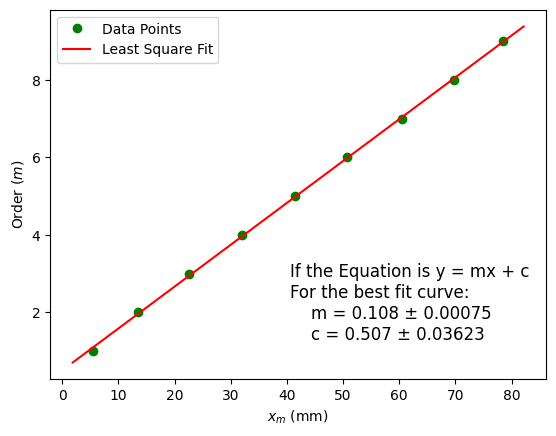
\includegraphics[width=0.37\textwidth]{graph_2.png}
	% 		\caption{\textbf{Graph for Second dataset}}
	% 		\label{graph:2}
	% 	\end{figure}

		% \begin{table}[H]
	\centering
	\resizebox{\columnwidth}{!}{%
	\begin{tabular}{|c|c|c|c|c|c|c|}
	\hline
	Drop no & Sl no & \begin{tabular}[c]{@{}c@{}}Free Fall\\ time (s)\end{tabular} & \begin{tabular}[c]{@{}c@{}}Mean Free fall\\ time ($t_f$) (s)\end{tabular} & \begin{tabular}[c]{@{}c@{}}Mean free fall velocity\\ $(v_f = \sfrac{L}{t_f}$\\ $\times 10^{5}\;(ms^{-1})$\end{tabular} & Balancing voltage(V) & Voltage (V) \\ \hline
	\multirow{5}{*}{1} & 1 & 4.9 & \multirow{5}{*}{4.64} & \multirow{5}{*}{0.0002} &  & \multirow{5}{*}{238} \\ \cline{2-3} \cline{6-6}
	 & 2 & 4.6 &  &  & 238 &  \\ \cline{2-3} \cline{6-6}
	 & 3 & 4.5 &  &  & 238 &  \\ \cline{2-3} \cline{6-6}
	 & 4 & 4.4 &  &  & 238 &  \\ \cline{2-3} \cline{6-6}
	 & 5 & 4.8 &  &  & 238 &  \\ \hline
	\multirow{4}{*}{2} & 1 & 11.5 & \multirow{4}{*}{11.275} & \multirow{4}{*}{9E-05} &  & \multirow{4}{*}{306.3333} \\ \cline{2-3} \cline{6-6}
	 & 2 & 11.2 &  &  & 306 &  \\ \cline{2-3} \cline{6-6}
	 & 3 & 11.3 &  &  & 306 &  \\ \cline{2-3} \cline{6-6}
	 & 4 & 11.1 &  &  & 307 &  \\ \hline
	\multirow{4}{*}{3} & 1 & 10.6 & \multirow{4}{*}{10.125} & \multirow{4}{*}{1E-04} &  & \multirow{4}{*}{230} \\ \cline{2-3} \cline{6-6}
	 & 2 & 10.3 &  &  & 230 &  \\ \cline{2-3} \cline{6-6}
	 & 3 & 9.8 &  &  & 229 &  \\ \cline{2-3} \cline{6-6}
	 & 4 & 9.8 &  &  & 231 &  \\ \hline
	\multirow{4}{*}{4} & 1 & 15.7 & \multirow{4}{*}{15.15} & \multirow{4}{*}{7E-05} &  & \multirow{4}{*}{360} \\ \cline{2-3} \cline{6-6}
	 & 2 & 14.7 &  &  & 360 &  \\ \cline{2-3} \cline{6-6}
	 & 3 & 15.3 &  &  & 359 &  \\ \cline{2-3} \cline{6-6}
	 & 4 & 14.9 &  &  & 361 &  \\ \hline
	\multirow{4}{*}{5} & 1 & 13.6 & \multirow{4}{*}{13.525} & \multirow{4}{*}{7E-05} &  & \multirow{4}{*}{264} \\ \cline{2-3} \cline{6-6}
	 & 2 & 13.1 &  &  & 266 &  \\ \cline{2-3} \cline{6-6}
	 & 3 & 13.9 &  &  & 264 &  \\ \cline{2-3} \cline{6-6}
	 & 4 & 13.5 &  &  & 262 &  \\ \hline
	\multirow{4}{*}{6} & 1 & 13.8 & \multirow{4}{*}{13.95} & \multirow{4}{*}{7E-05} &  & \multirow{4}{*}{407.6667} \\ \cline{2-3} \cline{6-6}
	 & 2 & 14.1 &  &  & 407 &  \\ \cline{2-3} \cline{6-6}
	 & 3 & 13.7 &  &  & 409 &  \\ \cline{2-3} \cline{6-6}
	 & 4 & 14.2 &  &  & 407 &  \\ \hline
	\end{tabular}%
	}
	\caption{Balancing Method Data}
	\label{tab:2}
\end{table}